\chapter{Conclusiones y trabajo futuro}
\noindent

\section{Conclusiones}
En este proyecto se ha realizado una aplicación que ayuda a gestionar la dieta de un deportista, pudiendo elegir una dieta entre las creadas por otros usuarios. 

Los deportistas pueden crear dietas que posteriormente pueden ser seguidas por otros usuarios. Además los deportistas, tienen la posibilidad de consultar la información detallada de cada uno de los alimentos que deben de consumir durante la realización de la dieta. A su vez, se pueden subir documentos explicativos para que el deportista que sigue la dieta conozca la finalidad cada alimento dentro de la dieta, pudiendo aportar mayor información al usuario.

Se puede valorar la dieta actual para que otros deportistas tenga referencias de ella, pudiendo a su vez, hacer comentarios sobre la dieta seguida.

% A pesar de que los integrantes no habían trabajado previamente con Android, ni habían desarrollado aplicaciones similares para dispositivos móviles, se considera que el servicio desarrollado aporta a los usuarios de la aplicación el valor que se había establecido al principio de la realización del proyecto, cumpliendo con los objetivos planteados al inicio.

En el siguiente enlace se puede ver y descargar, desde el repositorio de GitHub, el código del proyecto así como la aplicación ejecutable: \url{https://github.com/csegundo/Diet-Now}.

\section{Trabajo futuro}
% A continuación se van a describir una serie de implementaciones que se podrían añadir a la aplicación con el objetivo de mejorar la experiencia del usuario durante el uso de la misma.
A continuación se van a describir una serie de ideas de trabajo futuro que se podrían añadir a la aplicación con el objetivo de mejorar la experiencia del usuario durante el uso de la misma.

\begin{itemize}
    % \item \textbf{Modo oscuro:} la aplicación actualmente está implementada con el tema claro, el cual aparece configurado por defecto en numerosas aplicaciones. Son varias las motivaciones que nos pueden llevar a implementar esta mejora, destacando principalmente las siguientes.
    % \begin{enumerate}
    %     \item Comodidad visual: establecer un fondo oscuro en la aplicación como un color negro, gris o azul, disminuye el esfuerzo visual evitando que los ojos sufran de cansancio o fatiga. Además permite que se adapten con mayor facilidad a espacios con poca luminosidad.
    %     \item Ahorro de batería: en la mayoría de dispositivos móviles, el modo oscuro puede ayudar a reducir la batería entre un 14\% y un 60\%, dependiendo del brillo de la pantalla.
    % \end{enumerate}
    
    \item \textbf{Barra inferior de navegación:} el objetivo principal de esta implementación es la mejora de la experiencia del usuario, permitiéndole una navegación más sencilla e intuitiva entre las diferentes vistas añadiendo en la zona inferior de la pantalla un menú con una serie de iconos.% En la Figura \ref{fig:app_bottom_bars} se muestra un \textit{mockup} de dicho menú en dos vistas diferentes de la aplicación.
    % \begin{figure}[H]
    %     \centering
    %     \subfigure[Vista de la dieta actual]{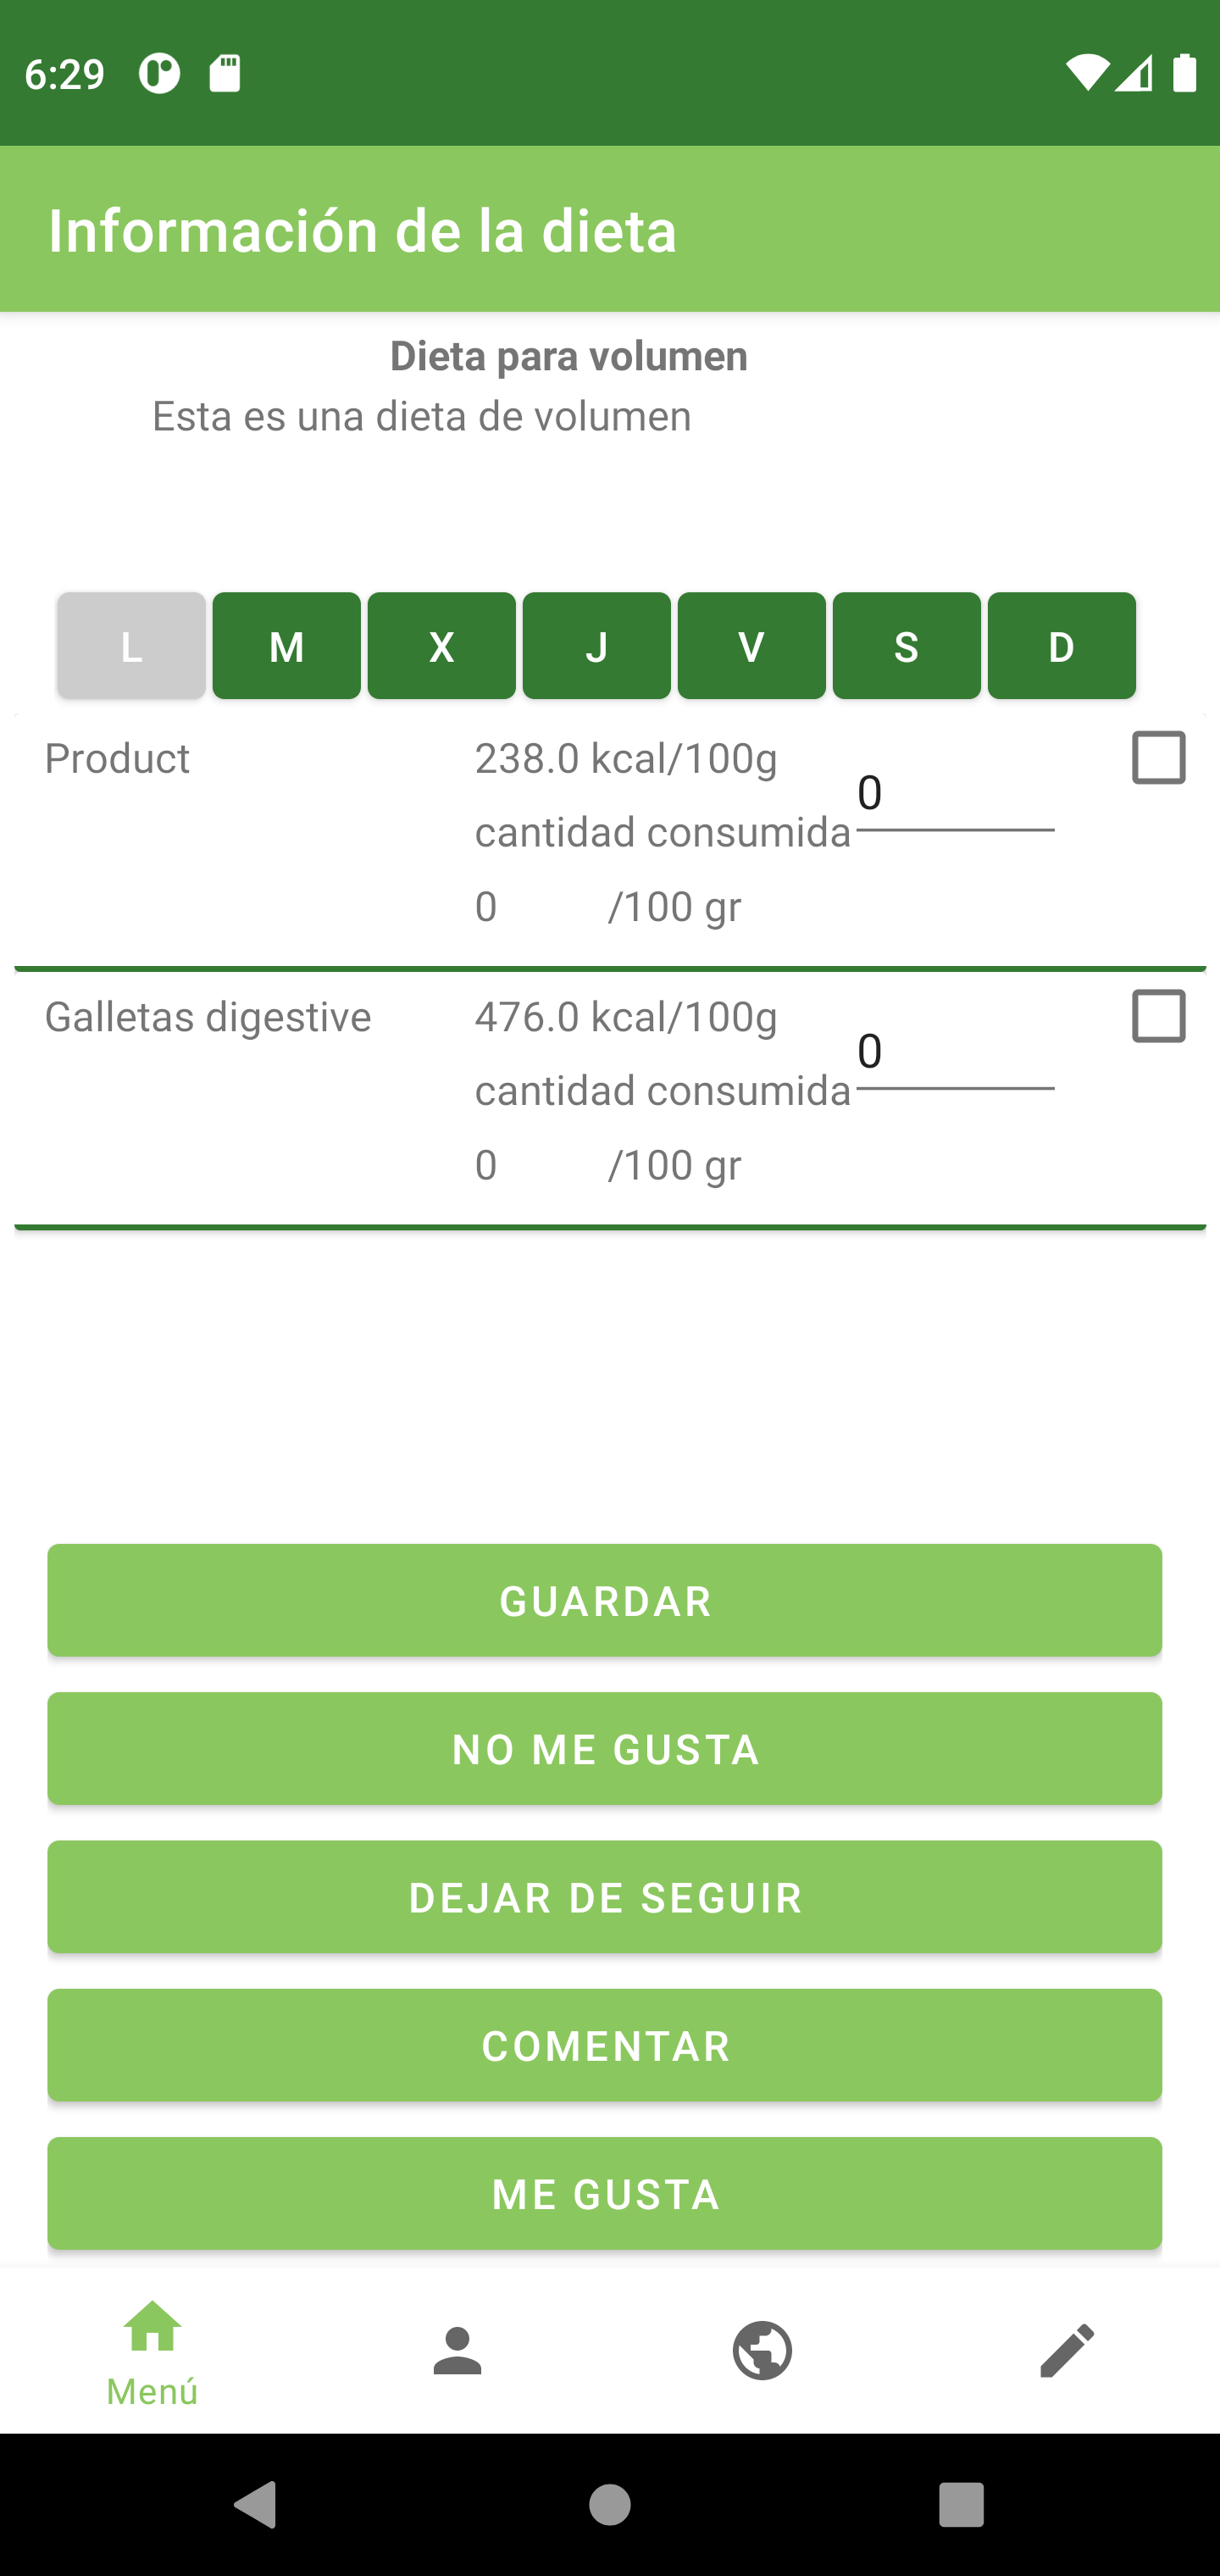
\includegraphics[width=0.45\textwidth]{Images/Capitulo9/bottomBar1.png}}
    %     \subfigure[Vista del perfil del deportista]{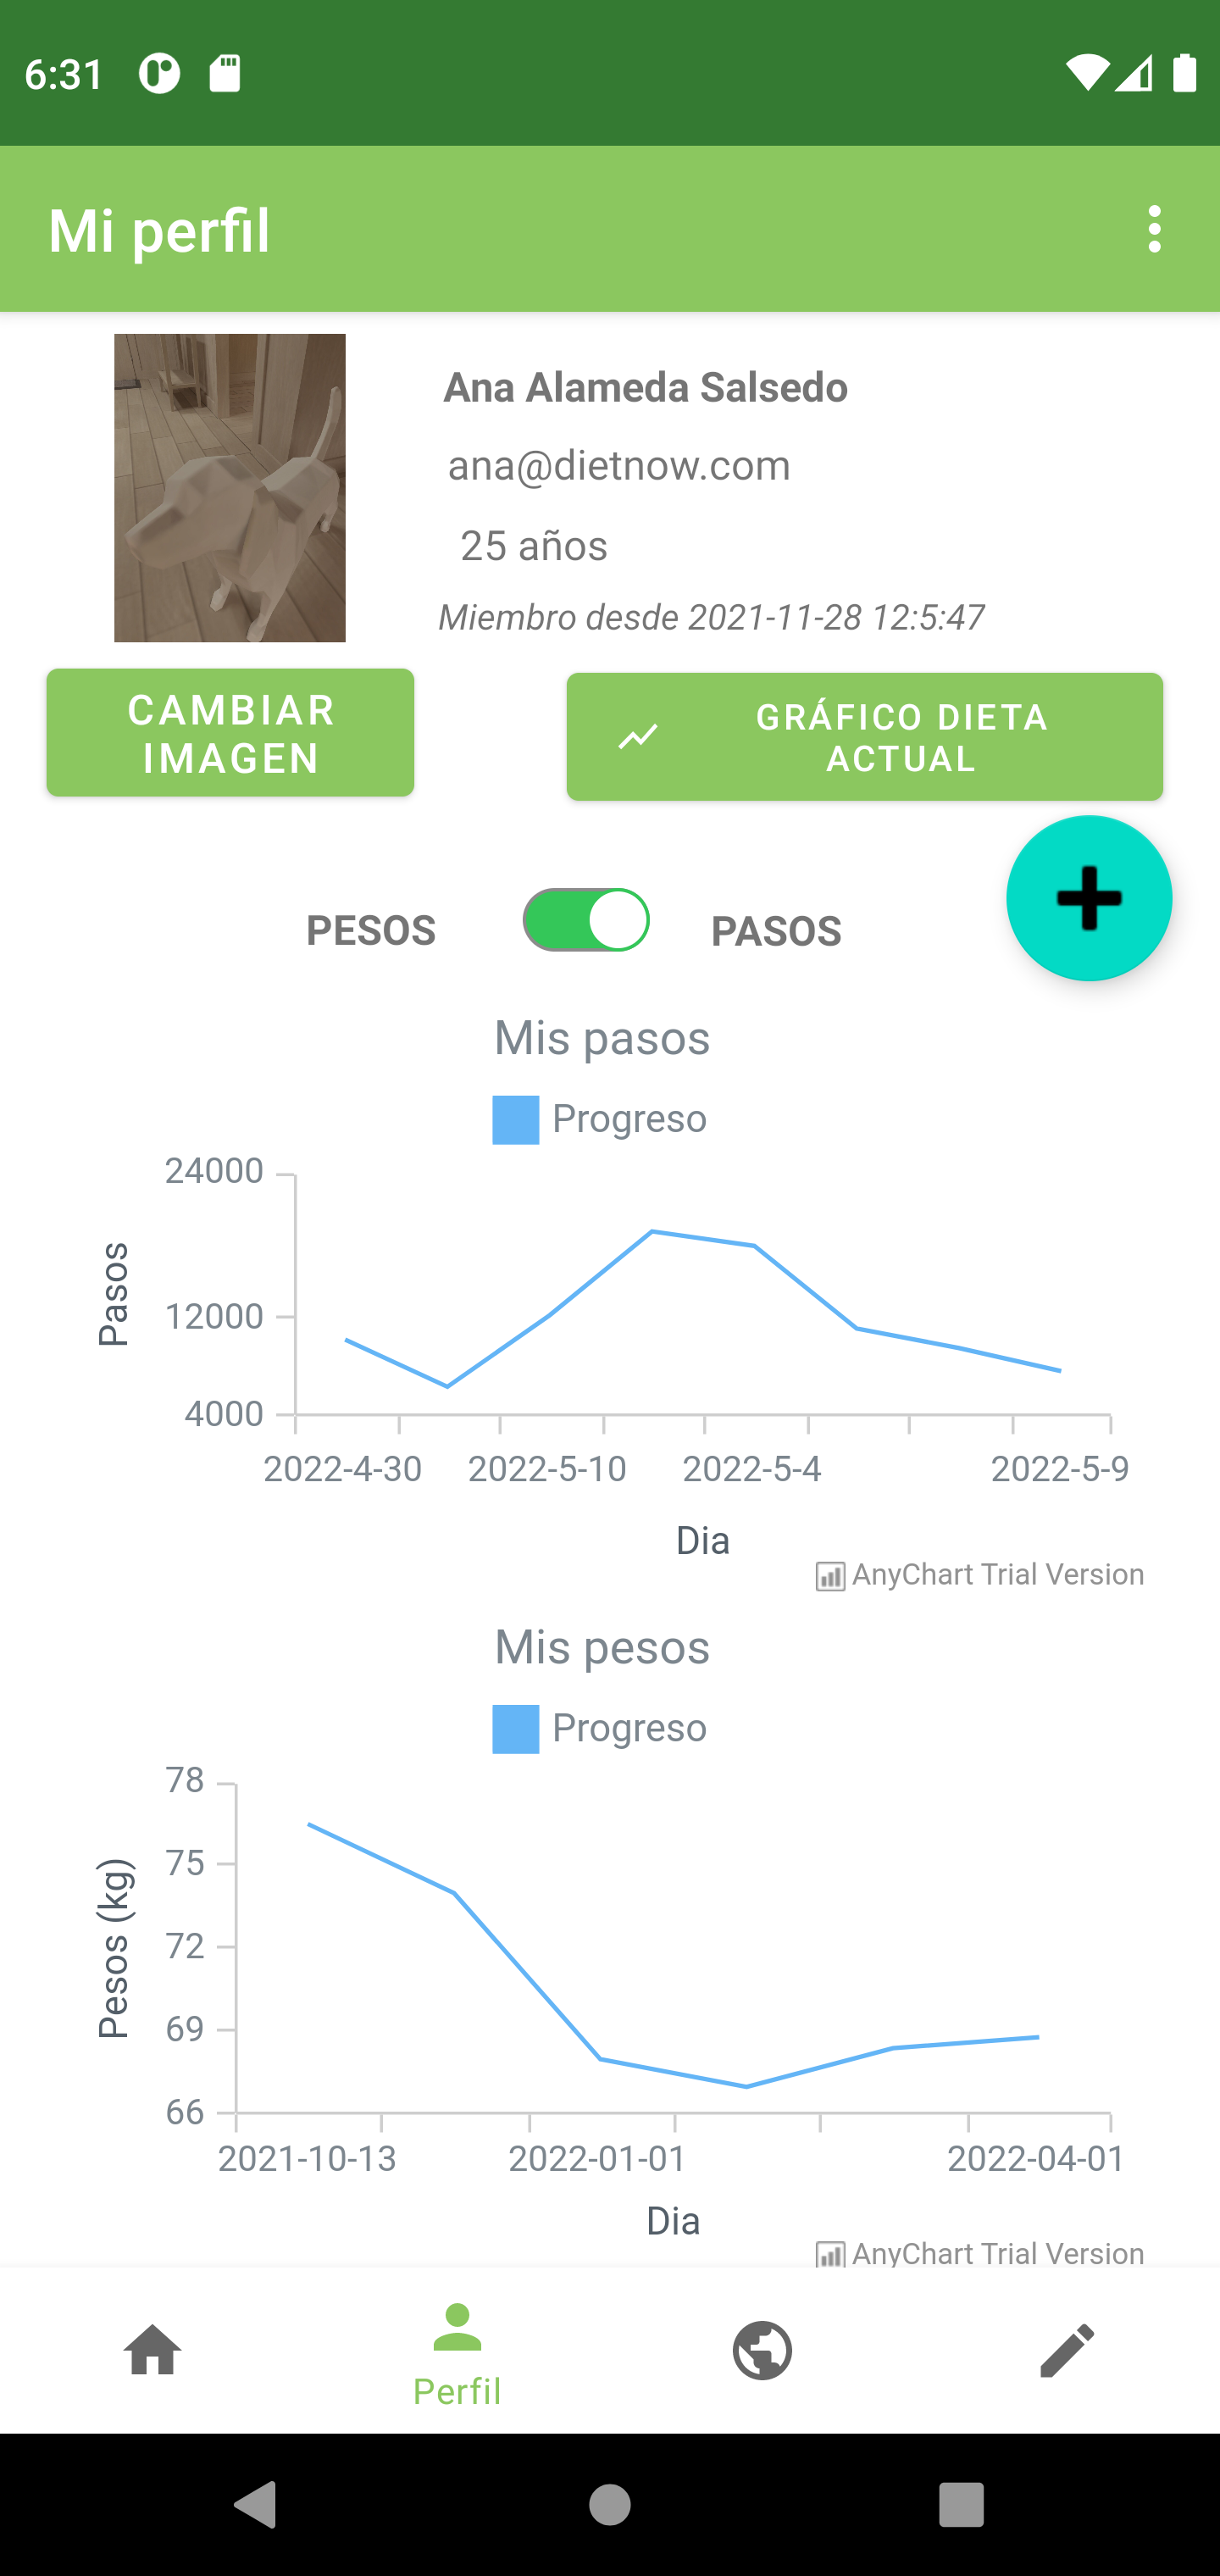
\includegraphics[width=0.45\textwidth]{Images/Capitulo9/bottomBar2.png}}
    %     \caption{\textit{Mockups} del menú inferior en diferentes vistas}
    %     \label{fig:app_bottom_bars}
    % \end{figure}
    
    % \item \textbf{Desplegar los servidores de \textit{Node.js} y \textit{Spring}:} para que la aplicación pueda llegar a todos los públicos, se podría desplegar tanto el servidor de \textit{Node.js} (que se encarga de llamar a la API de \textit{OpenFoodFacts}) como el servidor de \textit{Spring} (encargado de cambiar los campos del módulo de \textit{Firebase Authentication} y explicado anteriormente en la sección \ref{google_firebase_tools}). Una opción sería desplegar estos servidores en \textbf{\textit{Heroku}} \cite{heroku}, una plataforma como servicio (\textit{PaaS}) que nos permitiría realizar llamadas a estas APIs desde cualquier dispositivo ya que se encuentran en la nube y no de forma local.
    
    \item \textbf{Inicio de sesión con una cuenta de Google o Facebook:} para mejorar la usabilidad de la aplicación, se podría implementar esta nueva funcionalidad de inicio de sesión con una cuenta de Google o Facebook. Además del beneficio ya mencionado, podría aumentar considerablemente el número de usuarios en la aplicación debido a que la mayoría de usuarios de Facebook utilizan un dispositivo móvil, como se muestra en la Figura \ref{fig:fb_users}.
    \begin{figure}[H]
        \centering
        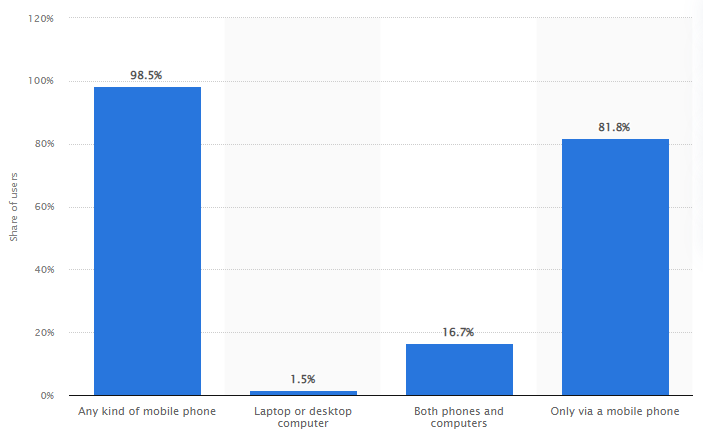
\includegraphics[width=\textwidth]{Images/Capitulo9/fbUsers.png}
        \caption{Dispositivos utilizados para iniciar sesión en Facebook en Enero de 2022 \cite{mobile_max_users}}
        \label{fig:fb_users}
    \end{figure}
    
    \item \textbf{Restablecer contraseña:} actualmente la aplicación no dispone de un sistema de recuperación de contraseña en el caso de que el usuario no recuerde la misma. Esta implementación facilitaría al usuario recuperar el acceso a su cuenta cuando olvida la contraseña, añadiendo un nuevo botón en la pantalla de inicio de sesión que envía un correo electrónico al email del usuario para que éste pueda restablecer la contraseña desde un enlace.
    
    \item \textbf{Añadir alimentos en grupo de comidas:} dar la posibilidad al deportista de añadir alimentos a una dieta en cada una de las cinco comidas que se realizan a lo largo del día. Cuando se va a añadir un alimento a una dieta, el usuario especifica si ese alimento pertenece al desayuno, comida, merienda...
    
    \item \textbf{Compartir dietas:} permitir a los usuarios que usen la aplicación la posibilidad de compartir mediante otras redes sociales o de mensajería las diferentes dietas insertadas en la aplicación.
    
    \item \textbf{Conexión con pulseras inteligentes:} ofrecer la posibilidad al usuario de conectar una pulsera o reloj inteligente a la aplicación. Mediante esta conexión, se pueden recopilar datos como el número de pasos caminados durante el día e introducirlos de forma automática en la cuenta del usuario para que se muestren en la gráfica de los pasos.
    
    \item \textbf{Conectar la gestión de dietas con asistente Alexa o Google:} permitir a los usuarios que deseen crear una dieta la posibilidad de hacerlo mediante voz. Esta herramienta se podría utilizar también para generar una compra mediante el asistente de Alexa o Google con los productos almacenados de una dieta.
    
\end{itemize}